\documentclass[legalpaper,10pt]{article}
\usepackage[left=1.50cm, right=1.50cm, top=1.50cm, bottom=1.50cm]{geometry}
\usepackage{multicol}
\usepackage{graphicx}
\usepackage{amsmath,amsfonts,amssymb}

\setlength{\columnsep}{1cm}
\title{\textbf{\LARGE{Optics}} \\ Interference,  Diffraction, Polarization}
\author{prepared by Shanku}

\begin{document}
\maketitle
\begin{multicols*}{2}

	\section*{Huygens Principal}
	According to Huygens, a light source in a \textit{homogeneous isotropic medium} sends out light in every direction \& these waves travel with equal velocity to carry energy with them to be transmitted in all directions.
	\begin{enumerate}
		\item {Every point on a given wavefront may be regarded as the source of a new disturbance, called \bf{secondary wavelets.}}
		\item The secondary wavelets(spherical) from each point spread out in all directions with the velocity of light.
		\item The envelope of these wavelets in the forward direction at any instance constitutes the new wave front at the instance.
	\end{enumerate}
	\paragraph{Wavefront-}defined as a \textit{surface} on which the phase of the disturbance is the same at any given instant of time. (two types = spherical /cylindrical)
	\paragraph{Huygens Principal can}
	\begin{itemize}
		\item Refraction \& reflection. Double Refraction in crystals.
		\item Explain polarization phenomena.
	\end{itemize}
	\paragraph{Huygens Principal cannot}
	\begin{itemize}
		\item Geometrical shadow theory.
		\item Diffraction interference.
	\end{itemize}

	\subsection*{Path Difference vs Phase Difference}
	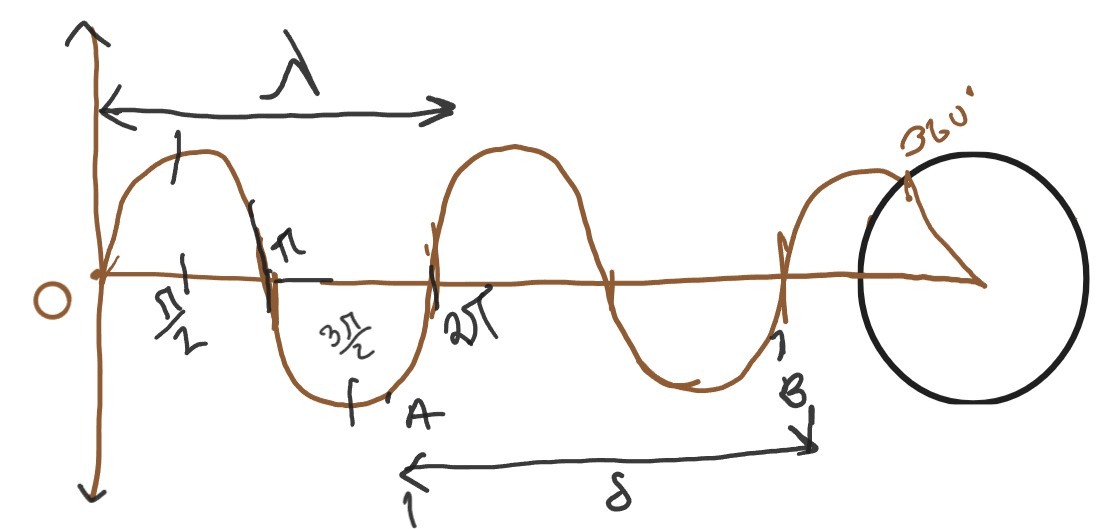
\includegraphics[width=7cm]{abc.png}
	Suppose 2 points $A\,and\,B$\par
	path difference $OB-OA=\delta$\par
	let, Phase difference $=\theta$\\
	we know if the difference between two waves equals to its wavelength($\lambda$) then $\theta=2\pi\,[360^{\circ}]$\par
	for path distance $\lambda$ phase diff $=2\pi$\par
	for path distance $\delta$ phase diff $=\dfrac{2\pi}{\lambda}\delta$\\
	\indent so, \(\mathbf{\boxed{\theta=2\pi\delta/\lambda }}\)

	\paragraph{Coherent Source:}the phase diff between the interfering waves must be zero or constant.

	\section*{Interference}
	\paragraph{Superposition}stats that.. the resultant disturbance of two or more waves acting on the same point simultaneously is the vector sum of the individual waves(disturbances).\\
	\indent	\( 	\text{Let, }y_1=a\sin{\omega t},  \text{ and } \,y_2=a\sin{(\omega t+\theta)}, \\ \)
	\indent\( 	\text{so, resultant will, } \)
	\begin{align*}
		y= & y_1+y_2
		\\= &a[\sin{\omega t}+\sin{(\omega t+\theta)}]
		\\= &2a \sin{(\omega t+\frac{\theta}{2}) \cos{\frac{\theta}{2}}}
		\\= &A \sin{(\omega t+\frac{\theta}{2})}
	\end{align*}


	\paragraph{Interference of light - the phenomenon where  \textit{monochromatic} light waves coming from two or more \textit{coherent sources}  Superimpose,  This leads to regions of constructive interference (brighter) and destructive interference (darker), creating an interference pattern.}

	\subsection*{Young's Double slit Experiment}
	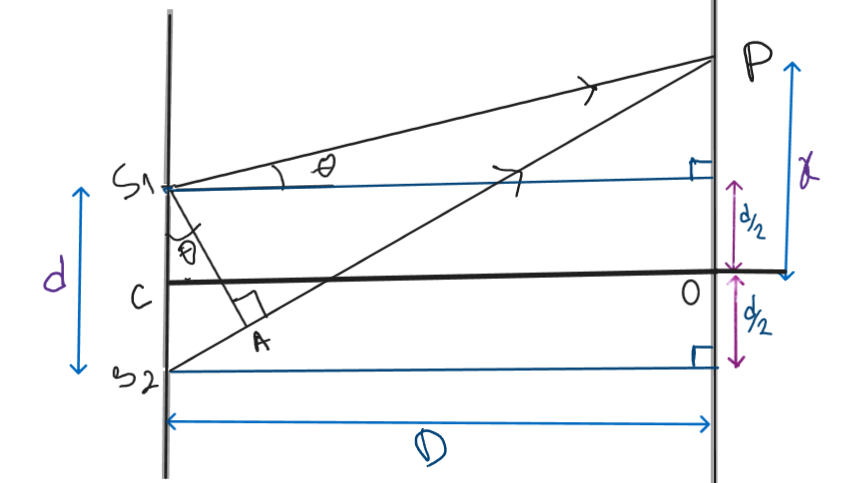
\includegraphics[width=9cm,height=4cm]{young1.png}\\
	\begin{math}
		\hspace*{1.5cm} l_1^2  =D^2+(x-d/2)^2
		\\\hspace*{1.5cm} l_2^2 =D^2+(x+d/2)^2
		\\\indent\text{  so, }(l_1+l_2)(l_1-l_2)=(x-d/2)^2 -(x+d/2)^2
		\\\indent\implies (l_1-l_2)\,2D=2xd
		\\\indent\implies l_1-l_2= path\, difference,\\
		\\\hspace*{3cm}\therefore \;\boxed{\bf{\delta=x_nd/D}}\\
	\end{math}
	% \pagebreak
	\\or, another way,\\
	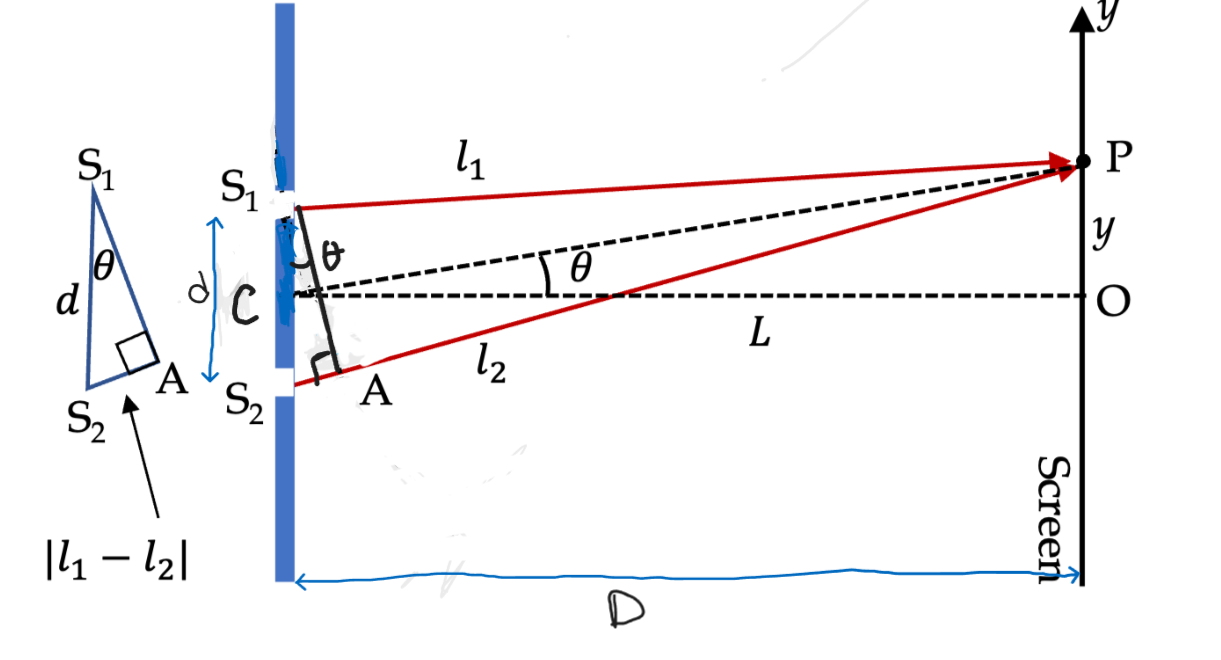
\includegraphics[width=9cm,height=4cm]{young2.png}\\
	\begin{math}
		\\\indent S_2A=\delta = S_1P-S_2P=l_1-l_2,\quad (D=CP)
		\\\indent\text{and in }\triangle S_1AS_2, \quad \sin{\theta}=S_2A/{S_1S_2}
		\\\indent\hspace*{2cm} \text{or,}\indent S_2A=\delta=d\sin{\theta}
		\\\indent P \,\& \,O \text{ are very close when, }  S_1P \approx S_2P \approx D
		\\\indent\text{as }[d<<D]\text{ and $y$ is very small}
		\\\indent\text{then, }\theta=\angle{S_2S_1A}=\angle{PCO}
		\\\therefore \quad \delta = d \sin\theta=\dfrac{dy}{PC}\approx \dfrac{dy}{D}\;  [if,\,S_1S_2=2d\implies \dfrac{2dy}{D}]
	\end{math}\\
	\\
	\large\textbf{now}, \textit{from principle of interference we know, resultant amplitude }
	$$A=2a\cos{\left(\dfrac{\theta}{2}\right)}=2a\cos{\left(\dfrac{2\pi\delta}{2\lambda}\right)}$$
	\textbf{for bright fringe,} \\
	\indent$A=max\implies2a\cos{(\theta/2)}=1$\\
	\indent so, $\theta=n\pi $ and $ \delta=n\lambda $\\
	\textbf{for dark fringe,} \\
	\indent$A=min\implies2a\cos{(\theta/2)}=0$\\
	\indent so, $\theta=(2n+1)\pi $ and $ \delta=(2n+1)\lambda $\\
	where [$n=0,1,2,3,4\dots $]

	\subsubsection*{Determination of fringe width:}
	spacing between $ nth$ \& $(n+1)th $ fringe will be,
	\begin{align*}
		x_n-x_{n-1} & =\frac{(n+1)\lambda D}{d}-\frac{n\lambda D}{d} \\
		x_n-x_{n-1} & = \boxed{\beta=\frac{\lambda D}{d}}
	\end{align*}

	\subsubsection*{Conditions for sustained interference:}
	\begin{itemize}
		\item must be coherent(same $\lambda$ or $\theta$),\\so we \textbf{can't use two real sources} they can't be coherent.(also $a_1\ne a_2$)
		\item same frequency($f$) or wavelength($\lambda$).\\\textbf{so,} if we cover slits with different transparent color paper that's lead to $\lambda_a \ne \lambda_b$
		\item if Polarized, then must be in same state of Polarization
		\item medium matters cause in water,\\ \(\beta'=\dfrac{D{\lambda}'}{d} = \beta'=\dfrac{D}{d}\dfrac{\lambda}{\mu}\)\\ so, $\beta{'} < \beta$ ,means width will reduced.
	\end{itemize}
	\subsubsection*{Conditions for good observation:}
	\begin{itemize}
		\item \(d\) must be small,\\\textbf{but if \({d<\lambda}\)} then $\beta$ is extremely large, lead to an \textbf{uniform illumination} got \textbf{no visible fringes}. \([\beta\propto(\lambda/d)]\)
		\item \(D\) should be relatively large. \(\beta \varpropto  D \)
		\item Background should be darker.
	\end{itemize}
	\subsubsection*{Conditions for good  contrast:}
	\begin{itemize}
		\item amplitudes should be equal or very nearly equal \(I_{m} \propto (a_1 \pm a_2)^2\; \text{  so, }a_1 \approxeq a_2\)
		\item the sources must be narrow
		\item sources must be monochromatic or very nearly so.
	\end{itemize}
	\paragraph*{Conservation of energy in interference:}In case of constructive interference, $I=I_{max}$ and bright fringes are formed in the screen. Whereas in case of destructive interference, $I=I_{min}$, dark fringes are formed.
	\par This implies that in interference and diffraction pattern, the intensity of light is simply being redistributed \textbf{i.e. energy is only transferred from dark to bright fringe and no energy is created or destroyed in the process.}
	\begin{align*}
		I_\text{total} & = I_1 + I_2                             \\
		               & = I_1 + I_2 + 2\sqrt{I_1 I_2}\ \cos\phi
	\end{align*}


	\section*{Diffraction}
	\textbf{The phenomenon of bending of light waves around obstacles or (aperture of sizes comparable with the wavelengths of light) \& resulting thereby in their spreading in \textit{Geometrical shadow} of the object is known as Diffraction.}
	\par It is a fundamental phenomenon in wave physics that occurs with all types of waves, including sound waves, electromagnetic waves (such as visible light, X-rays, and radio waves), and even matter waves (such as electrons and neutrons).
	\subsection*{Types of diffraction}
	\begin{description}
		\item[1. Fresnel type] the source and the screen \textit{(i.e. the point of observation)} or both are at finite distance from the obstacle or the aperture.
		\item[2. Fraunhofer type]  both source and screen are \textit{at $\infty$ distance }from each other.
	\end{description}
	\subsection*{Analytical treatment}
	\begin{math}
		\indent\text{path difference, }\delta=l_1-l_2,
		\\\indent\text{and in }\triangle S_1AS_2, \quad \sin{\theta}=S_2A/{S_1S_2}
		\\\indent\hspace*{2cm} \text{or, }\delta=a\sin{\theta}\quad (a=d)
		\\\indent\text{so, phase difference, }\phi=\dfrac{2\pi}{\lambda}\delta=\dfrac{2\pi}{\lambda} a\sin{\theta}\\
	\end{math}
	\indent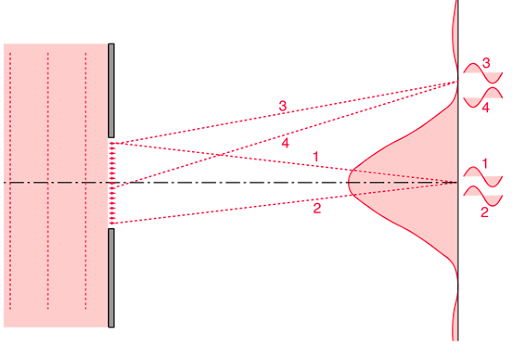
\includegraphics[width=8.5cm,height=3.5cm]{dif2.png}

	\textbf{for minima,} \\
	\hspace*{1cm}$a\sin{\theta}=n\lambda \quad [n=\pm1,\pm2\dots]$\\
	\hspace*{1cm}so, $ \delta = n\lambda \quad and, \quad \phi=n\pi$

	\textbf{for central maxima,}\\
	\hspace*{1cm}$ \delta=0,\quad so, a\sin{\theta}=0 $

	\textbf{for secondary maxima,} \\
	\hspace*{1cm}$a\sin{\theta}=(2n+1)\lambda/2 \quad [n=\pm1,\pm2\dots]$\\
	\hspace*{1cm}so, $ \delta = (2n+1)\lambda/2 \quad and, \phi=(2n+1)\pi/2$

	\textbf{so, central fringe width,}\\
	\hspace*{1cm}$\sin\theta=n\lambda/d=x_n/D, \quad so, x = \dfrac{n\lambda D}{a} $\\
	\hspace*{1cm}for, central fringe, $ 2x=\dfrac{2\lambda D}{a}\quad (n=1) $

	as $ \theta $ is small so $ \sin\theta=\theta $

	\textit{\textit{\textbf{for angular width}}} $ \theta=\lambda/a $\\

	\indent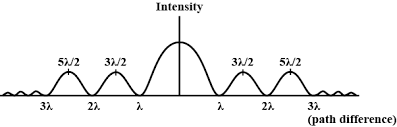
\includegraphics[width=8cm]{patt.png}

	\paragraph{\large The key aspects of diffraction are:}
	\begin{itemize}
		\item $ fringewidth \propto \lambda $ . so, for red light $ (\lambda \uparrow) $ central width high$\uparrow$,\\ same as for violet light $\downarrow$ width low $\downarrow$.
		\item if a $\downarrow$ then x $\uparrow$
		\item if monochromatic light used then we get a good contrast.
	\end{itemize}


	\section*{Interference vs Diffraction}
	\begin{description}
		\item[1. interaction occurs between: ]In interference , it's two separate wave-fronts originating from two coherent source\\
		In diffraction, it's among secondary wavelets originating from different points of the exposed part of the same wavefront.
		\item[2. The widths: ] fringes in interference may or may not be equal.\\But in diffraction they will never equal.
		\item[3. The regions of minimum intensity:] In interference they are perfectly dark.\\But not so in case of diffraction.
		\item[4. maxima:] are of uniform intensity in interference.\\ But the bright bands are of varying intensities in diffraction.
	\end{description}

	\section*{Polarization}
	\par\textbf{Polarization is a property of transverse waves which specifies the geometrical orientation of the oscillations.}
	\par In a transverse wave, \textit{the direction of the \underline{oscillation} is perpendicular to the direction of \underline{motion} of the wave.} \\

	\par\textbf{light} is a transverse electromagnetic wave consisting of vibrating electric and magnetic field. \textit{\textbf{the dominating electric vector is defined as \underline{light vector}.}}
	
	\begin{description}
		\item[Unpolarized light:]light waves vibrating in all possible directions. \textit{perpendicular to the direction of propagation.}
		\item[Polarized light:] light waves that are oriented in a specific direction, meaning the light waves vibrate in a particular plane.
		\item[Plane of vibration:] polarized light-waves vibrates in this plane.
		\item[Plane of polarization:] plane perpendicular to the plane of vibration.
		\item[Isotropic medium:] the physical properties of light are same in all direction.\textit{[glass,water]}
		\item[Anisotropic substances:] particularly crystals (except those with cubic symmetry) the physical properties are different in different direction. \\\textit{[calcite, quarts, tourmaline]}
		\item[O-Ray:] obey laws of refraction.
		\item[E-Ray:] extraordinary ray, doesn't obey laws.
	\end{description}

	\subsection*{Types of Polarization}
	\begin{enumerate}
		\item \textbf{Linear polarization:} The electric field of the light waves oscillates in a single plane.
		\item \textbf{Circular polarized light-} produced by \textit{two plane polarized light} vibrating perpendicular to each-other; where, amplitude and frequency equal but phase differ by $ \pi/2 $.
		\item \textbf{Elliptically polarized light-} produced if the amplitude and phase differ in previous case.
	\end{enumerate}

	\subsection*{Production of plane polarized light}
	By-- (1)reflection, (2)refraction, (3)double-refraction \&  (4)dichroism.
	\subsubsection*{Brewster's Law}
	the \textit{tangent of angle of polarization} equals the \textit{refractive index} of refractive medium. $$\boxed{ \mu=\tan i_p} $$
	\begin{itemize}
		\item angle of polarization \textbf{depends on} wave-length of light-wave.
		\item when light is incident at polarized angle, the \textit{plane of vibration} being at right angles to the\textit{ plane of incidence}.
	\end{itemize}
	let take, incident angle $ i_p $ is angle of polarization \& $ r $ is the angle of refraction.\\
	from Brewster's law, $ \tan i_p=\mu $\\
	also from snail's law, $ \mu=\sin i_p/\sin r $\\
	\indent so we get,\\
	\hspace*{2cm}$ \tan i_p=\dfrac{\sin i_p}{\sin r} \implies\cos i_p=\sin r$
	\hspace*{5cm}$ \implies i_p=90^\circ-r$\\\\
	\indent so, the reflected beam is perpendicular to refractive beam $ (i_p+r=\pi/2) $.
	
	\subsubsection*{Double Refraction}
	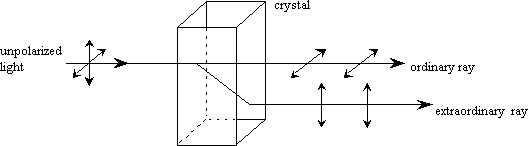
\includegraphics[width=8.3cm]{pol}
	\textit{The optical phenomenon of splitting of a single incident ray of non-polarized light into two refracted E-rays and O-rays(vibrates in principal section) when passing through anisotropic substances known as Double Refraction.}
	
	\subsubsection*{Dichroism: Polaroids}
	The selective absorption Some doubly refractive crystals absorbs one of O/E ray strongly \& allows other to pass by. (tourmaline) \\
	\indent When a film of\textit{ polyvinyl alcohol} \textit{heated \& stretched} 3-5 times it's original length, then it's molecules orients with long axis along the direction of stress. Then the film is \textit{saturated with iodine} =\textbf{ H-Polaroids.}\\
	\indent when the stretched polyvinyl alcohol heated with a catalyst(HCL) instead = \textbf{K-Polaroid.}


\end{multicols*}
\end{document}
